\section{Previsão de cargas. NBR 5410}

\begin{frame}{Norma NBR 5410}
	\begin{block}{Introdução}
		\begin{itemize}
			\item A norma NBR 5410 é a que estudaremos. Toda norma NBR é instituída pela \textbf{ABNT}, que se baseia em \textbf{padrões internacionais} para garantir o \textbf{consenso} do padrão brasileiro com o resto do mundo, assim como a \textbf{segurança} e \textbf{facilidade de entendimento} por todos.
			\item Essa norma se aplica à todas as instalações que usam tensão \textbf{abaixo} de \SI{1000}{\volt} de tensão alternada, de no máximo \SI{400}{\hertz}, ou \SI{1500}{\volt} de tensão contínua, já que esses são os limites para a \textbf{baixa tensão}.
			\item No Brasil, usamos a frequência de \SI{60}{\hertz} em nossas redes, que foi fixada por \textbf{decreto nacional}.
			\item A frequência da rede pouco influi sobre nossos estudos, mas pense nela como ``a quantidade de vezes que a tensão completa um ciclo de positivo/negativo a cada segundo''.
		\end{itemize}
	\end{block}

\end{frame}


\begin{frame}{Norma NBR 5410}
	\begin{block}{}
		$ \SI{60}{\hertz}=60 $ repetições dessa a cada segundo.
	\end{block}

	\centering
	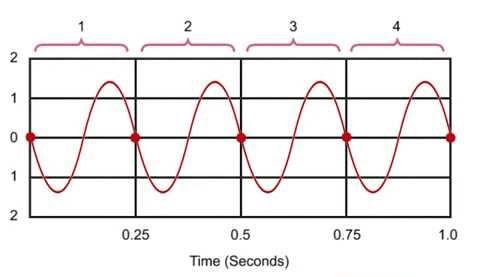
\includegraphics[width=0.7\linewidth]{Figuras/Ch02/fig1}

\end{frame}


\begin{frame}{Norma NBR 5410 - Projeto}
	\begin{block}{Noções iniciais - Projeto}
		\begin{itemize}
			\item  O projeto elétrico é a representação \textbf{gráfica} e \textbf{escrita} das \textbf{futuras instalações elétricas residenciais}.
			\item É onde serão definidos e indicados os \textbf{pontos de iluminação}, as \textbf{tomadas}, os \textbf{interruptores}, os \textbf{circuitos elétricos}, a posição do \textbf{quadro de distribuição} e dos \textbf{dispositivos de proteção}, levando em conta os equipamentos e aparelhos a serem usados pelos moradores de uma casa.
			\item Ele leva em consideração o \textbf{ambiente} e as suas \textbf{necessidades}, ou seja, \textbf{quantos} equipamentos serão ligados naquele cômodo e \textbf{quais} são os seus tipos.
			\item Em resumo, um sistema elétrico residencial visa suprir as \textbf{necessidades dos moradores}, seguindo os \textbf{padrões de segurança}, objetivando \textbf{economia} e \textbf{bom funcionamento}.
			\item O projeto também deve ser \textbf{acessível}, \textbf{flexível} e ter \textbf{capacidade de reserva}.
		\end{itemize}
	\end{block}

	%	\centering
	%	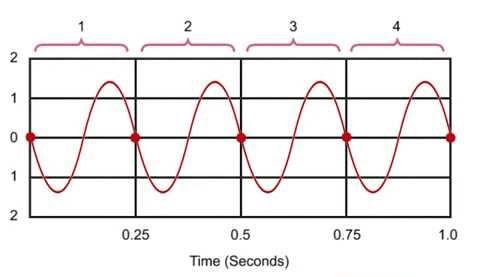
\includegraphics[width=0.7\linewidth]{Figuras/Ch02/fig1}

\end{frame}


\begin{frame}{Norma NBR 5410 - Projeto}
	\begin{block}{Noções iniciais - Projetista}
		\begin{itemize}
			\item Para o \textbf{projetista}, a solução procurada visa \textbf{atender a uma necessidade}.
			\item No caso dessa disciplina, estudaremos como estabelecer de que forma a \textbf{energia elétrica} será conduzida da \textbf{rede de distribuição} até os \textbf{pontos de utilização} em um determinado edifício, abrangendo todos os aspectos envolvidos.
			\item O projeto é, portanto, uma \textbf{mediação entre duas situações} ou \textbf{dois estados}.
		\end{itemize}
	\end{block}

	\bigskip

	\centering
	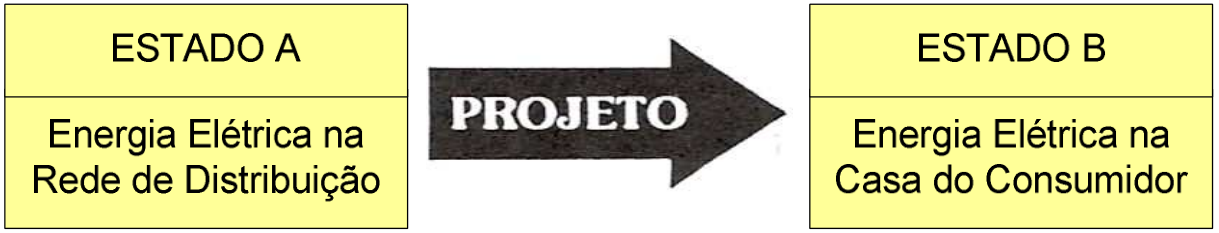
\includegraphics[width=0.7\linewidth]{Figuras/Ch02/fig4}


\end{frame}


\begin{frame}{Norma NBR 5410 - Projeto}
	\begin{block}{Aprofundamento - Projeto}
		\begin{itemize}
			\item É importante ter em mente que \textbf{a solução não é única}.
			\item Frequentemente, existirão \textbf{diversas alternativas} de soluções possíveis.
			\item O projetista deverá \textbf{examiná-las}, avaliar as possibilidades de cada uma delas, e finalmente \textbf{escolher} aquela que julgar a \textbf{mais adequada}.
			\item \textbf{Nem sempre} esta escolha é \textbf{fácil}.
			\item O \textit{projeto} é, em essência, uma \textbf{antecipação detalhada }de uma \textbf{solução }que será implementada para \textbf{satisfazer} determinado \textbf{objetivo}.
			\item Por esta razão, o projetista deve preocupar-se com a sua \textbf{viabilidade}, tanto do ponto de vista \textbf{técnico}, como do ponto de vista \textbf{econômico}.

		\end{itemize}
	\end{block}
	%	
	%	\centering
	%	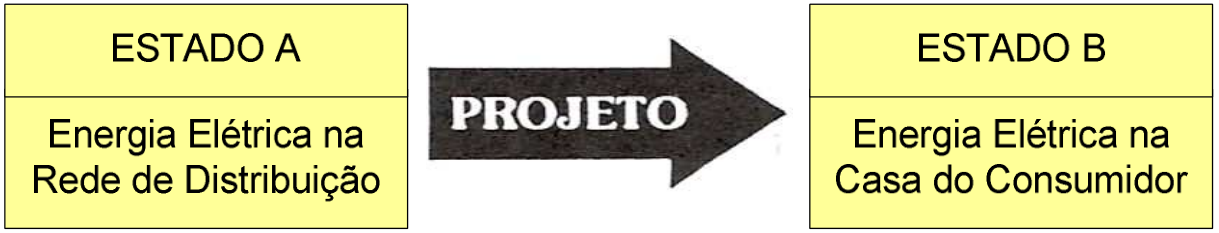
\includegraphics[width=0.7\linewidth]{Figuras/Ch02/fig4}


\end{frame}


\begin{frame}{Norma NBR 5410 - Projeto}
	\begin{block}{Aprofundamento - Projeto}
		\begin{itemize}
			\item Tendo em mente que em boa parte das ocasiões o projetista \textbf{não }estará \textbf{presente }na \textbf{implantação do projeto}, ele deve questionar-se: o projeto é \textbf{perfeitamente compreensível}? O projeto está \textbf{suficientemente detalhado}?
			\item Um projeto é o resultado de uma interação dos sujeitos envolvidos: \textbf{cliente}, \textbf{profissional projetista }e \textbf{entidades normatizadoras }(associações normatizadoras, órgãos do poder público, concessionárias, etc).
		\end{itemize}
	\end{block}

	\centering
	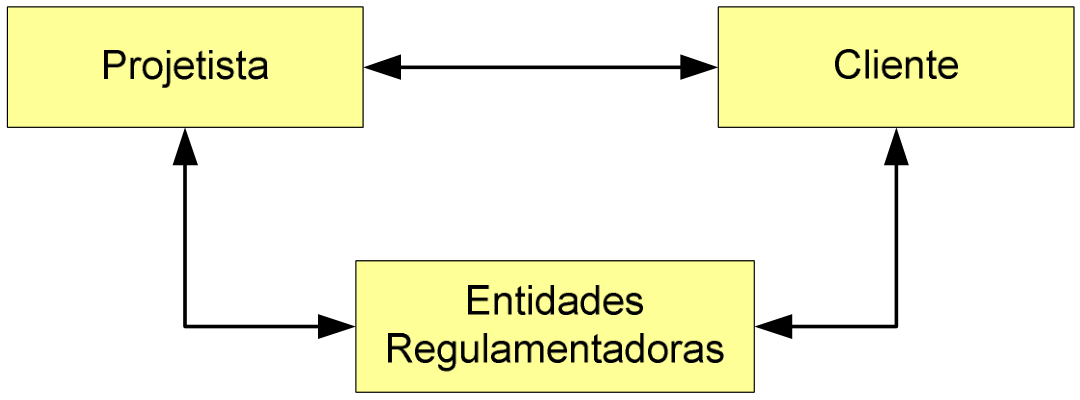
\includegraphics[width=0.6\linewidth]{Figuras/Ch02/fig5}

\end{frame}


\begin{frame}{Norma NBR 5410 - Projeto}
	\begin{block}{Aprofundamento - Projeto}
		\begin{itemize}

			\item Um projeto é dinâmico, portanto, pode sofrer \textbf{revisões}.
			\item Qualquer revisão deve ser devidamente \textbf{analisada}, \textbf{aprovada} pelo \textbf{projetista} e \textbf{registrada}.
			\item É importante observar que uma revisão que ocorre na fase de execução tende a ser mais cara do que se houvesse ocorrido na fase de projeto, uma vez que poderá implicar em \textbf{desperdício }de recursos \textbf{materiais}, recursos \textbf{humanos} e \textbf{tempo}.

		\end{itemize}
	\end{block}

	%	\centering
	%	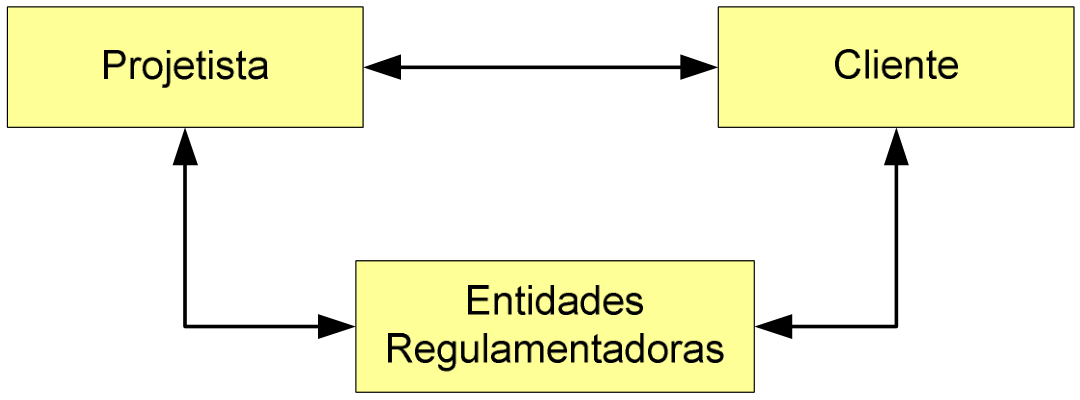
\includegraphics[width=0.7\linewidth]{Figuras/Ch02/fig5}


\end{frame}


\begin{frame}{Norma NBR 5410 - Projeto}
	\begin{block}{CREA}
		\begin{itemize}
			\item Atualmente, as atividades no âmbito da engenharia já estão contempladas pelo Código de Ética Profissional publicado pelo sistema \textbf{CONFEA} e \textbf{CREA}'s.
			\item Para o desempenho profissional de suas atividades, o projetista deverá obter \textbf{habilitação específica} através de \textbf{formação} em \textbf{centros educacionais especializados} (universidades, faculdades de engenharia, centros de educação tecnológica, escolas técnicas etc.) e \textbf{registro} no respectivo \textbf{Conselho Profissional}.
			\item O registro profissional, no caso de cursos superiores e cursos técnicos da área de engenharia, junto ao CREA --- Conselho Regional de Engenharia, Arquitetura e Agronomia --- confere ao profissional a habilitação necessária, especificando as \textbf{áreas} e os \textbf{limites} de suas \textbf{atribuições profissionais}.
		\end{itemize}
	\end{block}
\end{frame}


\begin{frame}{Norma NBR 5410 - Projeto}
	\begin{block}{CREA e ART}
		\begin{itemize}
			\item Segundo definição do próprio CREA, a função deste é atuar em \textbf{defesa da sociedade contra os maus profissionais}, e \textbf{não} como \textbf{associação de classe}, como poderia nos parecer a princípio.
			\item Para a defesa dos \textbf{interesses} dos \textbf{técnicos} e \textbf{engenheiros} existem as \textbf{Associações} e \textbf{Sindicatos}.
			\item Para garantir aos profissionais registrados nos CREA's um meio de \textbf{cadastrar }suas \textbf{obras }e \textbf{serviços}, \textbf{cargos }ou \textbf{funções}, \textbf{cursos }e \textbf{prêmios}, foi criada, em 1977, a Anotação de Responsabilidade Técnica (ART), através da Lei nº 6.496/77.
		\end{itemize}
	\end{block}
\end{frame}


\begin{frame}{Norma NBR 5410 - Projeto}
	\begin{block}{ART}
		\begin{itemize}
			\item A ART \textbf{define}, para efeitos legais, os \textbf{responsáveis técnicos pelo empreendimento}, \textbf{obra} ou \textbf{serviço}, tendo valor de \textbf{um contrato}. Mas para isso, ela deve ser registrada no CREA onde for executada a \textbf{atividade técnica}.
			\item Cada projeto terá o seu respectivo \textbf{registro} junto ao CREA, através da ART. Nesta ocasião, o Conselho \textbf{verificará} se o profissional está \textbf{habilitado} para aquela \textbf{especialidade}, fazendo a respectiva anotação que passará a constar do \textbf{acervo técnico} do profissional.
			\item A ART descreve o \textbf{objeto do projeto}, o qual, na forma da \textbf{legislação em vigor}, estará sob a \textbf{responsabilidade do técnico}.
		\end{itemize}
	\end{block}
\end{frame}


\begin{frame}{Norma NBR 5410 - Projeto}
	\begin{block}{Objetivos da ART}
		\begin{enumerate}[a]
			\item Garantia da qualidade dos serviços prestados;
			\item Formação de currículo;
			\item Acervo técnico;
			\item Garantia de mercado de trabalho;
			\item Garantia de honorários/salários;
			\item Licitações;
			\item Aposentadoria;
			\item Salário Mínimo Profissional – SMP;
			\item Delimitação de responsabilidade profissional;
			\item Fiscalização de honorários.
		\end{enumerate}

	\end{block}

	%	\centering
	%	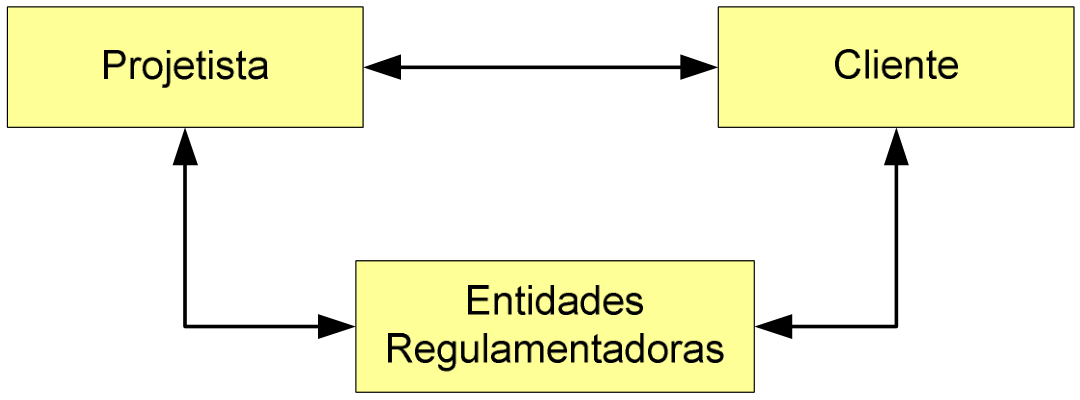
\includegraphics[width=0.7\linewidth]{Figuras/Ch02/fig5}


\end{frame}

\begin{frame}{Norma NBR 5410 - Projeto}
	\begin{block}{Habilitação}
		\begin{itemize}
			\item Os profissionais habilitados para as atividades de elaboração e execução de projetos de instalação de energia elétrica são os \textbf{engenheiros} e os \textbf{técnicos industriais de nível médio}, conforme \textbf{atribuições específicas} definidas para cada categoria profissional.
		\end{itemize}
	\end{block}
\end{frame}


\begin{frame}{Norma NBR 5410 - Projeto}
	\begin{block}{Partes componentes de um projeto}
		%		Sendo a representação escrita de uma instalação, o projeto consiste basicamente em desenhos e documentos. De uma maneira geral, em um projeto de instalações elétricas de edifícios de uso coletivo, temos as seguintes partes:
		\begin{itemize}
			\item ART;
			\item Carta de solicitação de aprovação à concessionária;
			\item Memorial descritivo;
			\item Memorial de cálculo (cálculo da demanda, dimensionamento de condutores, condutos e proteções);
			\item Plantas (planta de situação, planta de pavimentos);
			\item Esquemas verticais (prumadas);
			\item Quadros (quadros de distribuição de cargas, diagramas);
			\item Detalhes (entrada de serviço, caixa seccionadora, centros de medição, caixas de passagem, aterramentos, outros);
			\item Convenções;
			\item Especificações;
			\item Lista de materiais.
		\end{itemize}
	\end{block}

	%	\centering
	%	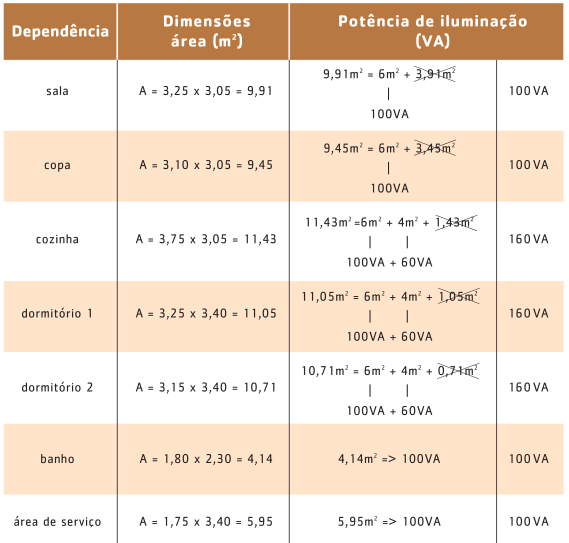
\includegraphics[height=0.6\textheight]{Figuras/Ch02/fig2}

\end{frame}


\begin{frame}{Norma NBR 5410 - Projeto}
	\begin{block}{Cálculo}
		\begin{itemize}
			\item Dispostas as \textbf{partes do projeto}, é necessário aprender a fazê-lo \textbf{efetivamente}.
			\item Um técnico ou engenheiro que venha a executar o trabalho deve saber \textbf{dimensionar} corretamente os \textbf{componentes} que serão utilizados na instalação, e poderá fazer isso através de \textbf{cálculos}.
			\item É a \textbf{norma NBR 5410} que dispõe as \textbf{regras} para a definição das \textbf{potências} em uma casa, e até de \textbf{quantas fases} serão necessárias.
			\item Pode parecer bastante \textbf{complexo} e distante, mas se você perguntar a \textbf{engenheiros} e \textbf{eletricistas}, verá que este é um assunto \textbf{cotidiano} em suas vidas.
		\end{itemize}
	\end{block}

	%	\centering
	%	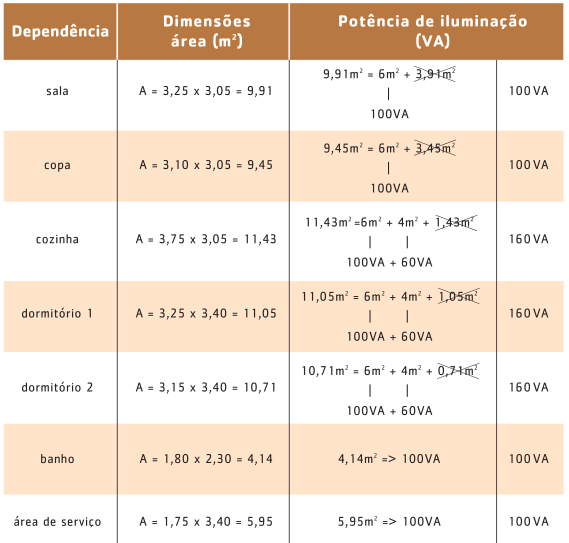
\includegraphics[height=0.6\textheight]{Figuras/Ch02/fig2}

\end{frame}


\begin{frame}{Norma NBR 5410 - Projeto}

	\centering
	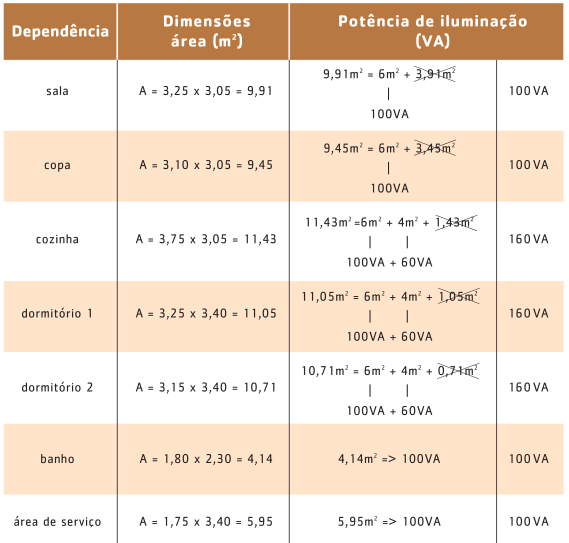
\includegraphics[height=0.9\textheight]{Figuras/Ch02/fig2}

\end{frame}


\begin{frame}{Norma NBR 5410 - Projeto}
	\begin{block}{Componentes}
		Para realizar uma instalação elétrica, é importante saber alguns \textbf{conceitos}:
		\vspace{-0.45cm}
		\begin{itemize}
			\item As \textbf{instalações elétricas}, por exemplo, são um \textbf{conjunto de componentes elétricos} que têm como \textbf{finalidade} proporcionar a \textbf{utilização de energia elétrica}.
			\item Os \textbf{condutores} são os \textbf{fios} pelos quais a \textbf{corrente elétrica} passa. Esses condutores podem ser de \textbf{quatro tipos diferentes}: neutro, fase, retorno ou terra.
		\end{itemize}
	\end{block}
\end{frame}


\begin{frame}{Norma NBR 5410 - Projeto}
	\begin{block}{Componentes - Tipos de condutores}
		\begin{itemize}
			\item O \textbf{neutro} é um condutor \textbf{aterrado}, portanto não dá choque, já que tem um ddp de \SI{0}{\volt} em relação ao chão.
			\item Já a \textbf{fase} é um condutor que apresenta uma ddp, que pode ser de \SI{127}{\volt} ou de \SI{220}{\volt}. Enquanto isso, o \textbf{retorno} é um condutor utilizado nas instalações de \textbf{iluminação}, e liga o ponto de luz à tomada.
			\item O \textbf{terra}, também conhecido como \textbf{condutor de proteção}, é ligado a hastes cravadas na terra, além de acompanhar todos os circuitos e alguns equipamentos. Ele tem como função \textbf{proteger} os \textbf{equipamentos} ligados aos circuitos de \textbf{sobrecargas elétricas} e também os \textbf{usuários} de possíveis \textbf{choques elétricos}.
		\end{itemize}
	\end{block}
\end{frame}


\begin{frame}{Norma NBR 5410 - Projeto}
	\begin{block}{Apresentação da metodologia}
		\begin{itemize}
			\item Para fazer um projeto de instalações elétricas é importante começar pela análise da \textbf{planta baixa} do local.
			\item Nessa planta estarão contidas todas as \textbf{medidas dos ambientes e vãos} e é a partir dessas informações que serão calculados o \textbf{perímetro} e a \textbf{área} de cada ambiente. E não se preocupe em conseguir essa planta, ela é um documento básico da construção do imóvel.
			\item Com base no \textbf{perímetro} e na \textbf{área}, é possível saber a \textbf{quantidade mínima} da \textbf{potência de iluminação} e de \textbf{pontos de tomada} necessários \textbf{em cada cômodo}. Já ao associar \textbf{área} e \textbf{perímetro} com a \textbf{finalidade do ambiente}, é possível definir ou prever as \textbf{cargas} de \textbf{cada tomada}.
		\end{itemize}
	\end{block}
\end{frame}


\begin{frame}{Norma NBR 5410 - Projeto}
	\centering
	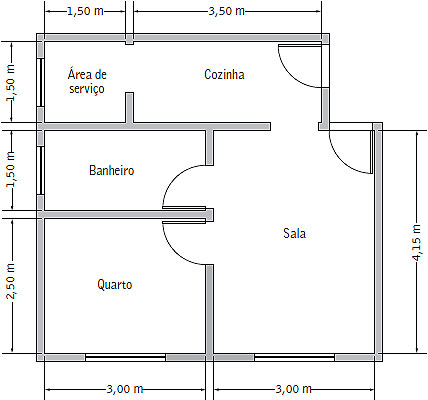
\includegraphics[width=0.7\linewidth]{Figuras/Ch02/fig3}

\end{frame}


\begin{frame}{Norma NBR 5410 - Projeto}
	\begin{block}{Previsão de cargas}
		\begin{itemize}
			\item A previsão de cargas se baseia na \textbf{análise de cada ambiente} e nas \textbf{necessidades das pessoas que utilizarão o espaço}.
			\item Por exemplo, se o quarto será usado como um escritório ou será utilizado por duas pessoas, as necessidades serão diferentes.
			\item O ideal é que o projeto atenda às duas hipóteses, porém, em situações em que a destinação do ambiente e a distribuição dos móveis \textbf{já estejam definidas}, é possível fazer uma \textbf{previsão} ainda mais \textbf{fiel} e \textbf{realista}.
		\end{itemize}
	\end{block}
\end{frame}


\begin{frame}{Norma NBR 5410 - Projeto}
	\begin{block}{Previsão de cargas}
		\begin{itemize}
			\item Por exemplo, em uma cozinha, é importante prever que serão utilizados alguns equipamentos, como geladeira, máquina de lavar louça, liquidificador, batedeira, entre outros, assim como os locais em que serão colocados.
			\item Para que o espaço seja \textbf{funcional}, é preciso \textbf{prever} os \textbf{locais} e \textbf{todas as potências} desses aparelhos, a fim de definir a \textbf{necessidade de cargas} do ambiente.
			\item A partir dessa \textbf{previsão de potências e cargas}, podem ser realizados os \textbf{cálculos} necessários para obter outras informações, como \textbf{bitolas dos condutores e eletrodutos}. Contudo, é preciso definir a \textbf{quantidade de pontos de iluminação e de tomadas} antes.
		\end{itemize}
	\end{block}
\end{frame}


\begin{frame}{Norma NBR 5410 - Projeto}
	\begin{block}{Previsão de cargas}
		\begin{itemize}
			\item Conforme falamos bastante até agora, é a partir da \textbf{área} e do \textbf{perímetro} que é determinado o \textbf{número mínimo} de \textbf{lâmpadas}, de \textbf{interruptores} e de \textbf{tomadas}. A partir dessas determinações, podem ser \textbf{separados os circuitos}.
			\item Esses devem ter as \textbf{cargas distribuídas entre si}, de forma que fiquem \textbf{equilibrados}, com \textbf{quantidade de carga parecida}. A NBR 5410 aconselha que os circuitos sejam \textbf{separados} em circuitos de \textbf{iluminação}, para \textbf{tomadas de uso geral} (TUG) e para \textbf{tomadas de uso específico} (TUE).
			      %			\item Lembre-se que você não precisa e não deve fazer isto sozinho. Com certeza, você precisa da ajuda de um profissional da área da construção civil para te auxiliar nessa etapa inicial.
		\end{itemize}
	\end{block}
\end{frame}


\begin{frame}{Norma NBR 5410 - Projeto}
	\begin{block}{Previsão de cargas}
		\begin{itemize}
			\item Quanto à iluminação, em cômodos com área \textbf{inferior a \SI{6}{\meter\squared}}, devem ser preditas cargas de, \textbf{pelo menos, \SI{100}{\va}}; já nos que têm área \textbf{superior a \SI{6}{\meter\squared}}, deve ser predita uma \textbf{carga mínima de \SI{100}{\va} para os primeiros \SI{6}{\meter\squared}} — contudo, \textbf{a cada aumento de \SI{4}{\meter\squared}}, devem ser somadas \textbf{mais \SI{60}{\va}}.
			\item Deve haver pelo menos \textbf{um ponto por cômodo} e, nos \textbf{banheiros}, as \textbf{luminárias} (arandelas) devem estar há, pelo menos, \textbf{\SI{60}{\centi\meter} do boxe}.
		\end{itemize}
	\end{block}
\end{frame}


\begin{frame}{Norma NBR 5410 - Projeto}
	\begin{block}{Previsão de cargas}
		\begin{itemize}
			\item Quanto às tomadas, cômodos com área \textbf{menor que \SI{6}{\meter\squared}} devem ter, \textbf{no mínimo, uma tomada com \SI{100}{\va}}, e cômodos com \textbf{área maior que \SI{6}{\meter\squared}} devem ter, \textbf{pelo menos, uma tomada de \SI{100}{\va} a cada \SI{5}{\meter} ou fração de perímetro}. Essas tomadas devem ser \textbf{distribuídas} de forma \textbf{mais uniforme possível}.
			\item Os banheiros devem ter \textbf{uma tomada de \SI{600}{\va} próxima ao lavatório}.
		\end{itemize}
	\end{block}
\end{frame}


\begin{frame}{Norma NBR 5410 - Projeto}
	\begin{block}{Previsão de cargas}
		\begin{itemize}
			\item Em \textbf{copas}, \textbf{cozinhas} e \textbf{áreas de serviço}, deve haver, \textbf{no mínimo, uma tomada a cada \SI{3.5}{\meter} ou fração de perímetro}.
			\item É necessário haver, \textbf{pelo menos, uma tomada acima das bancadas}, e para \textbf{as três primeiras tomadas}, devem ser atribuídas \textbf{cargas de \SI{600}{\va}}. \textbf{Para as demais} pode ser atribuída a carga de \textbf{\SI{100}{\va}}.
			\item Quando se trata de \textbf{subsolos}, \textbf{garagens}, \textbf{varandas} e \textbf{halls}, deve ser colocada, \textbf{no mínimo, uma tomada de \SI{1000}{\va}}, sendo que a \textbf{quantidade não será relacionada com o perímetro} do ambiente.
		\end{itemize}
	\end{block}
\end{frame}


\begin{frame}{Norma NBR 5410 - Projeto}
	\begin{block}{Previsão de cargas}
		\begin{itemize}
			\item Após essa etapa, podem ser traçados os \textbf{eletrodutos} que vão \textbf{conectar} as \textbf{tomadas}, \textbf{interruptores} e \textbf{iluminação} que \textbf{interligam um determinado circuito aos outros circuitos} e, posteriormente, ao \textbf{quadro de distribuição}.
			\item Esses \textbf{eletrodutos} podem passar pelo \textbf{piso}, pelo \textbf{teto} e pela \textbf{parede}, e \textbf{não deve ocorrer sobreposição}. Também é importante que estejam presentes na \textbf{quantidade adequada} para que os condutores \textbf{não fiquem acumulados} e ocorra \textbf{sobreaquecimento}.
		\end{itemize}
	\end{block}
\end{frame}


\begin{frame}{Norma NBR 5410 - Projeto - Exemplo \#01}
	\centering
	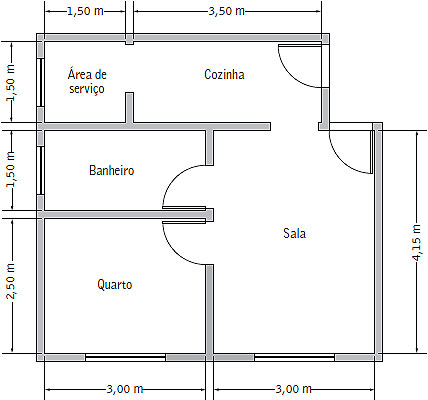
\includegraphics[width=0.7\linewidth]{Figuras/Ch02/fig3}
\end{frame}


\begin{frame}{Norma NBR 5410 - Projeto - Exemplo \#01}
	\begin{block}{Previsão de cargas}
		\centering
		\resizebox{1\textwidth}{!}{
			\begin{tabular}{lccccc}
				\toprule
				\multirowcell{2}[-3pt]{Ambiente} & \multicolumn{2}{c}{Dimensões} & \multirowcell{2}[-3pt][l]{Pontos de                            \\ Tomadas} & \multicolumn{2}{c}{Potência (\si{\va})}\\ \cmidrule{2-3}\cmidrule{5-6}
				                                 & Área (\si{\meter\squared})    & Perímetro (\si{\meter})             &   & Iluminação & Tomadas \\\midrule
				Sala                             & \num{12.45}                   & \num{14.3}                          & 3 & 160        & 300     \\
				Quarto                           & \num{7.5}                     & \num{11}                            & 3 & 160        & 300     \\
				Banheiro                         & \num{4.5}                     & \num{9}                             & 1 & 100        & 600     \\
				Cozinha                          & \num{5.25}                    & \num{10}                            & 3 & 160        & 1800    \\
				Área de serviço                  & \num{2.25}                    & \num{6}                             & 2 & 100        & 1200    \\ \bottomrule
			\end{tabular}}
	\end{block}
\end{frame}


\begin{frame}{Norma NBR 5410 - Projeto}
	\begin{block}{Previsão de cargas}
		\begin{itemize}
			\item Temos também as \textbf{TUE's}, que devem ser incluídas separadamente.
			\item A quantidade de TUE's é estabelecida de acordo com o número de aparelhos de utilização, com corrente nominal superior a \SI{10}{\ampere}.
		\end{itemize}
	\end{block}

	\centering
	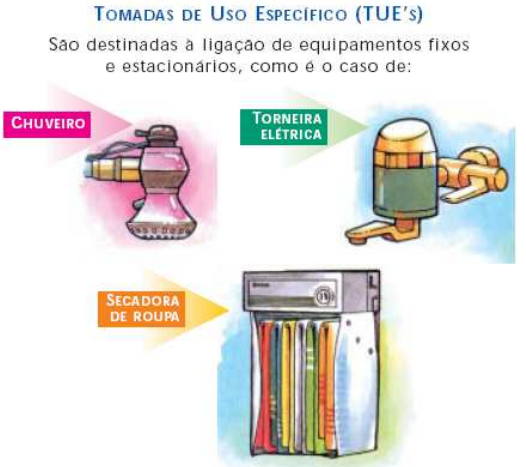
\includegraphics[width=0.5\linewidth]{Figuras/Ch02/fig6}

\end{frame}


\begin{frame}{Norma NBR 5410 - Projeto}
	\centering
	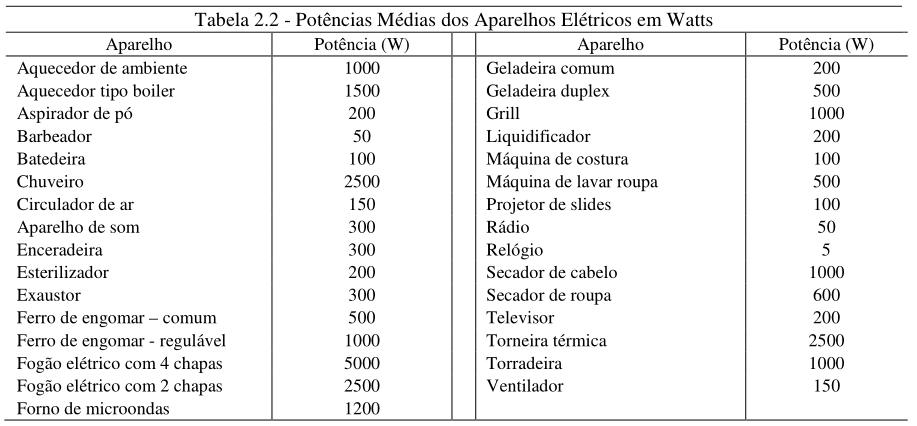
\includegraphics[width=1\linewidth]{Figuras/Ch02/fig7}
\end{frame}


\section*{Exercícios}
\frame{
	\frametitle{Exercícios}
	\begin{block}{}
		01. Dado um apartamento com dimensões:

		\begin{center}
			%			\resizebox{1\textwidth}{!}{
			\begin{tabular}{lccccc}
				\toprule
				\multirowcell{2}[-3pt]{Ambiente} & \multicolumn{2}{c}{Dimensões} &                         \\ \cmidrule{2-3}
				                                 & Área (\si{\meter\squared})    & Perímetro (\si{\meter}) \\ \midrule
				Sala                             & \num{36}                      & \num{24}                \\
				Quarto                           & \num{30}                      & \num{22}                \\
				Banheiro                         & \num{8.75}                    & \num{12}                \\
				Cozinha                          & \num{10}                      & \num{14}                \\
				Área de serviço                  & \num{2}                       & \num{6}                 \\ \bottomrule
			\end{tabular}%}
		\end{center}

		(a) Identifique a quantidade de pontos de tomadas em cada um dos cômodos.

		\medskip

		(b) Identifique as potências de iluminação em cada um dos cômodos.

		\medskip

		(c) Identifique as potências de tomadas em cada um dos cômodos.

	\end{block}
}

\section*{Referências}

\frame{
	\frametitle{Referências e Exercícios Complementares}
	\begin{itemize}
		\item CREDER, Hélio; Instalações Elétricas, 14ª edição, Editora LTC, Rio de Janeiro, 2004.
		\item Manual de Instalações Elétricas - Prysmian.
	\end{itemize}
	%\centering{\alert{Página 36 - \textbf{1.6.1 até 1.6.5, 1.6.17 até 1.6.19}}} \\
	%	\centering{\alert{Lista de exercícios 01}}
}